\documentclass[a4paper,12pt]{report}
% \renewcommand{\familydefault}{\sfdefault}
\usepackage[english]{babel}
\usepackage{blindtext}
\usepackage{microtype}
\usepackage{graphicx}
\usepackage{wrapfig}
\usepackage{enumitem}
\usepackage{lscape}
\usepackage{amssymb}
\usepackage{epstopdf}
\usepackage{algorithm}
\usepackage{algorithmic}
\usepackage{subfig}
\usepackage{float}
\usepackage{wrapfig}
\usepackage{fancyhdr}
\usepackage{amsmath}
\usepackage{index}
\usepackage{float}
\usepackage{titlesec}
\usepackage{cite}
\usepackage{relsize}
\usepackage{pdflscape}
\usepackage{cite}
\usepackage{geometry}
\usepackage{afterpage}
\usepackage[parfill]{parskip}
\usepackage{hyperref}

\graphicspath{ {./images/} }
\hypersetup{
    colorlinks,
    citecolor=black,
    filecolor=black,
    linkcolor=black,
    urlcolor=black
}

\title{\Huge{\textbf{Improving the Reliability of Artificial Intelligence}}\\
\vspace*{0.3cm}
\Large{Research Proposal}}

\titleformat{\chapter}[display]
    {\normalfont\bfseries}{}{0pt}{\huge}\author{Ajal Singh - 12621189\\
    Supervisor: Diep Nguyen}
\date{25 October, 2020}

\begin{document}
\maketitle
\tableofcontents
\listoffigures
\listoftables
\setcounter{page}{1}

%% Engineering Research Problem
\chapter{Engineering Research Problem}
\label{chap:chap1}

\section{Background }
As the use of Artificial Intelligence (AI) and Machine 
Learning (ML) continues to grow throughout the world 
in high-risk applications, models have become 
ever-increasingly complex and diverse. As a result, 
they often become prone to accidents where unintended 
and harmful behaviour is observed, and consequently are 
scrutinized as disruptive and unreliable solutions. The 
recent emergence in smart cities have seen AI and ML being 
used in various applications such as transportation, 
healthcare, environmental, and public safety as depicted in Figure 1.1.

\begin{figure}[h]
    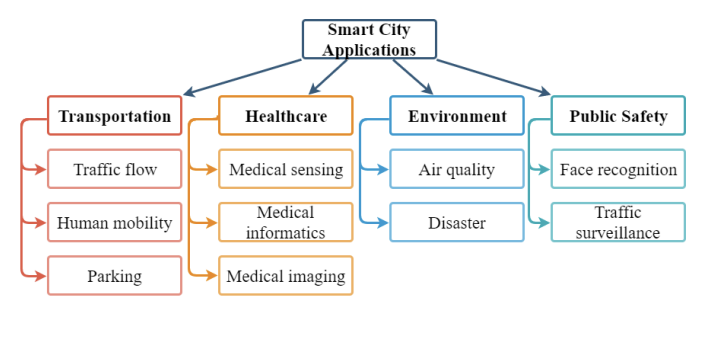
\includegraphics{smart_city_applications.png}
    \caption{Smart City Artificial Intelligence Applications \cite{chen}}
    \label{fig:smart}
\end{figure}

\enlargethispage{\baselineskip}
For an AI/ML system to be considered reliable, it must 
perform tasks when required as it was originally 
intended, produce consistent results using real-world 
data (and shifts in data), and remain robust and 
predictable. This means it must also fail in a 
predictable manner \cite{Saif}. 

\section{Applications}
One of the most discussed and disruptive applications of ML is facial 
recognition systems used by authorities which fails to distinguish 
between darker skin individuals. This technology is used to assist the 
police in identifying potential criminals/suspects and often leads to 
wrongful arrests of dark-skinned people \cite{Moutafis}. This example highlights the 
importance and the need for reliability in ML solutions. 

There are many more applications where reliability is crucial due to the 
potential consequences. Cancer diagnosis systems trialled in the US are 
failing to detect cancer in patients in differing hospitals and/or countries which may result 
in death. As another example, unintended behaviours in traffic management systems would 
increase congestion resulting in poor ambient air quality and noise 
pollution.

The rapid technological changes in manufacturing have produced a boom 
in Industry 4.0 applications involving Artificial Intelligence, connected
 devices (IoT) and Big Data. A paper on use cases of AI in Industry 4.0 
 summarises the advantages ML, \textit{“AI with machine learning technique can 
 automate the manufacturing process which increase the productivity, 
 efficiency, optimize production cost and reduce manual error” }\cite{9004327}. A 
 key area is predictive maintenance where real-time equipment data is 
 captured and historical equipment data is evaluated using AI and ML 
 models to estimate the equipment life cycle and hence perform timely 
 maintenance to reduce or eliminate down-time. Down-time is undesirable
for manufacturers as it equates to the loss of revenue.

AI in cybersecurity helps protect enterprises by detecting unusual 
activity, patterns, and malicious behaviour and can respond to different 
situations. For manufacturers, this could be used for asset protection 
while banks and financial institutions may use this form ML to detect suspicious 
activity and fraud \cite{9004327}. 

\section{Project Contextualisation}
A tutorial presented by Suchi Saria and Adarsh Subbaswamy of John Hopkins University \cite{saria2019tutorial} postulates some causes and failure prevention techniques for use in supervised learning systems (regression and classification). 
Some of the sources of unreliability discussed are the use of inadequate data, changes in training and deployment environments, and model misspecification. 
These aforementioned causes will form the basis of this research project.

Another reliability issue is discussed in a separate paper, \textit{‘Concrete Problems in AI Safety’} \cite{Amodei} is the prevalence of reward hacking in Reinforcement Learning systems. 
Reward hacking is the AI agent’s ability to cheat the system to achieve the highest reward in an unintended way. 
For example, a positive reward may be given to a traffic management system when there is no congestion. However, the AI model decides to divert all traffic through alternative routes essentially shutting down this particular road/intersection. 
This prevents congestion but does not perform as desired. This notion is also investigated in this research project.

\section{Research Question}
\noindent\rule{\linewidth}{0.4pt}
\begin{quotation}
\textit{How can the reliability of Artificial Intelligence be improved against 
inadequate data labelling, unsuitable algorithm choices, and reward 
hacking?}
\end{quotation}
\noindent\rule{\linewidth}{0.4pt}

%% Methodology
\chapter{Methodology}
This project has been divided into three main sections based on the factors of unreliability mentioned earlier in \hyperref[chap:chap1]{Section 1}. 
The main factors studied in this project are:
\begin{itemize}
    \item Label Bias and Environmental Datashift
    \item Suitable Algorithm Selection
    \item Reward Hacking
\end{itemize}

To prevent any delays, writing of the report will be completed 
concurrently with experimentation. This is to ensure that ideas, 
thoughts, results, and conclusions are fresh in mind at the time of 
writing. This will improve the quality of the report which is crucial 
as it should be a direct and official indication of all work completed. 
The report is also the only assessable task in 41030 – Engineering 
Capstone, and therefore the only way to gain marks.

\section{Label Bias and Environmental Datashift}
To investigate the effect of biased data labelling we will train two models using a single independent algorithm. 
One will use biased data while the other uses unbiased data. 
These datasets will be modelled using the mathematical framework outlined in the conference paper \textit{‘Identifying and Correcting Label Bias in Machine Learning’} \cite{Jiang}. 
Each model will be trained and evaluated using data which has been split from the same distribution. 
For a model to be considered reliable it must be able to properly generalise or adapt well to new and unseen data. 
A good, reliable model can achieve high accuracy scores with low variance between datasets. 
Therefore, both of these trained models will then be fed previously unseen data (i.e. deployment data) to determine its ability to generalize.

\section{Suitable Algorithm Selection}
As can be seen in Figure 2.1, when it comes to AI and ML, the appropriacy of solutions or algorithms depends on elements such as the specific application and the level of supervision required. 
More often than not, more than one algorithm could be a viable solution (see \hyperref[fig:algor]{Figure 2.2}). 
Therefore, to investigate suitable algorithm selections, models will be trained with a single dataset using different algorithms (with different assumptions). 
They will then be tested for accuracy to determine suitable algorithm choices. Evaluating the reliability of a model is dependant of the model type. 
Accuracy, precision and recall are three common metrics we can use to evaluate a model. 
However, depending on certain applications, other complex means of metric evaluation may be necessary. 

\begin{figure}[h]
    \centering
    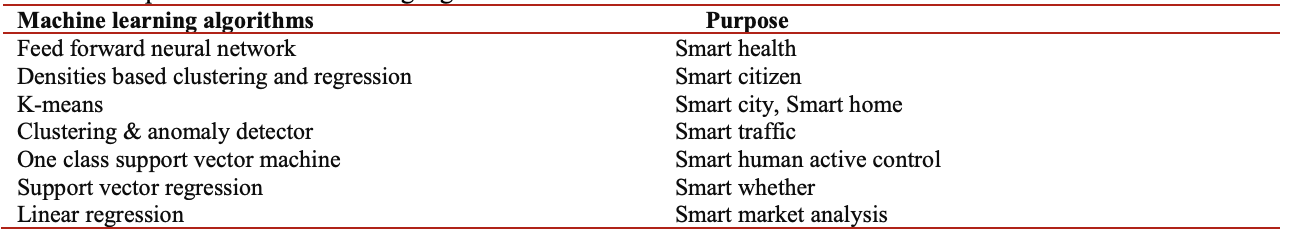
\includegraphics[width=1\textwidth]{ML algorithms.png}
    \caption{Machine Learning Algorithms for specific applications \cite{Mohapatra}}
    \label{fig:applic}
\end{figure}

The bias-variance trade-off should be considered when optimising ML models. 
Bias is the model’s ability to learn the wrong things due to oversimplification or incorrect assumptions. 
Variance is the error due to sensitivity as a result of small fluctuations in training data. 
As the complexity of the model increases, bias decreases but the variance will increase. 
This is the trade-off between these two factors. 
An overfit model is one that is too complex resulting in high variance and low bias, while an underfit model has low variance and high bias due to its simplistic nature. 
Both overfit and underfit models are undesirable and it is ideal to find a suitable trade-off between bias and variance (hence complexity) to yield a well fit model capable of adapting to different datasets \cite{Jedamski}. 

\begin{figure}[H]
    \centering
    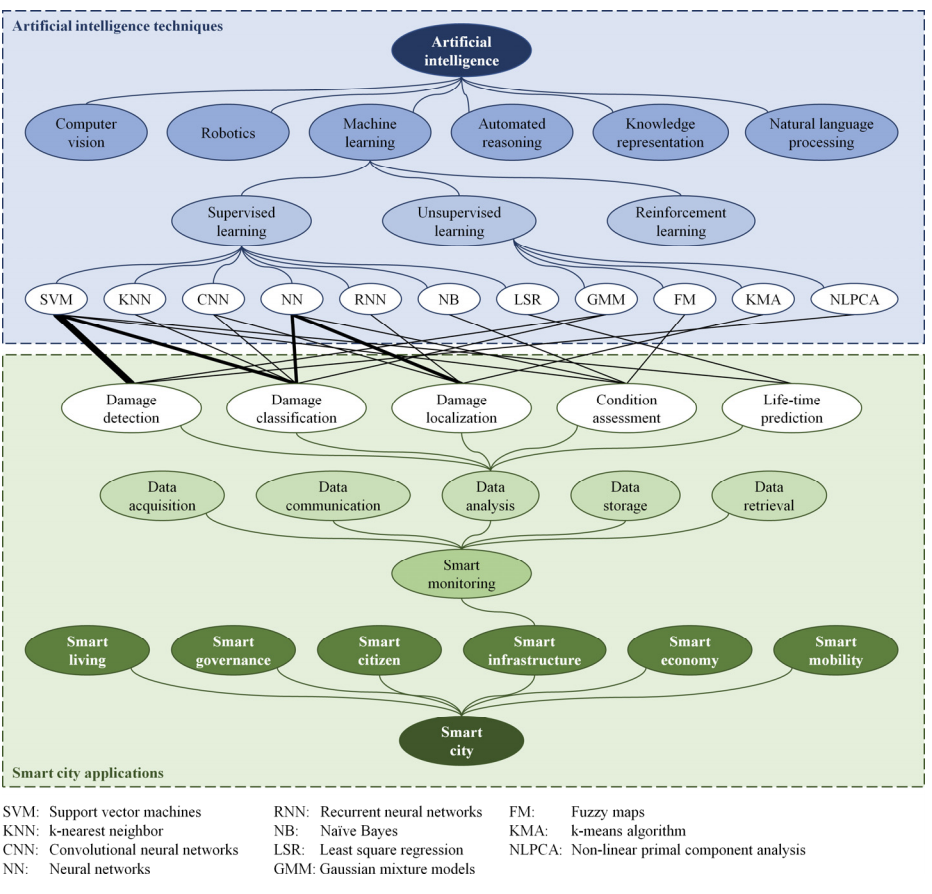
\includegraphics[width=\textwidth]{smart monitoring algorithms.png}
    \caption{Available ML algorithms for smart monitoring \cite{inproceedings}}
    \label{fig:algor}
\end{figure}

\enlargethispage{\baselineskip}
The dataset/s to be used in the above experiments will be obtained through various open-source data collections available online. 
Therefore, data collection is not a part of this project.
To ensure validity during the training of models, the data distribution will be split into three smaller datasets for training, validation and testing. 
The training set is used to train the models to fit the data and are evaluated against the validations set. 
The validation set being unseen, allows us to determine which models are generalising well to new examples. 
After the best model has been selected it is again tested on the test dataset as a final check on its generalisation ability. 
The training set accounts for 60\% of the full data set, while the validation and test sets account for 20\% each. 

\section{Reward Hacking}
The two unreliability factors discussed in the above experiments are concerned mainly with supervised learning models. 
A major reliability issue within reinforcement learning models is reward hacking. 
We will perform a systematic literature review on applications and known causes of unreliability due to reward hacking as well as potential solutions.

%% Project Management
\chapter{Project Management}
\section{Scope}
The scope of the project involves studying the factors that affect the reliability of Artificial Intelligence (AI) and Machine Learning (ML) with a focus on smart city applications. 
After specific applications have been identified, the factors affecting the reliability are investigated in detail before finally performing experiments to propose solutions to improve reliability. 
The factors studied within this project are data labelling and environmental data shifts, suitable algorithm selection, and reward hacking. 
The mathematics behind these factors will be researched before performing experiments in an attempt to propose solutions.

\section{Process and Timeline}
A Gantt chart has been produced to illustrate the order of completion of major and minor milestones involved in this project. 
This not only shows the duration of the whole project but also the time required for each milestone and its dependency on other tasks. 
The arrangement of milestones against specific dates acts as a schedule where each task has a required deadline which, ideally should be met to prevent delays. 
However, delays in most projects are unavoidable, therefore precautionary buffer periods have been added to allow flexibility in this project. \\

See \hyperref[sec:app2]{Appendix 2} for the Gantt Chart and detailed process including milestone deadlines. 

\newpage
\section{Milestones}
Tasks and activities involved in this project have been split into major and minor milestones as seen below in Figure 3.1. 
Major milestones are logically ordered towards the completion of the project and may consist of any number of smaller milestones. 

\begin{figure}[h]
    \centering
    \hspace*{-1.5cm}  
    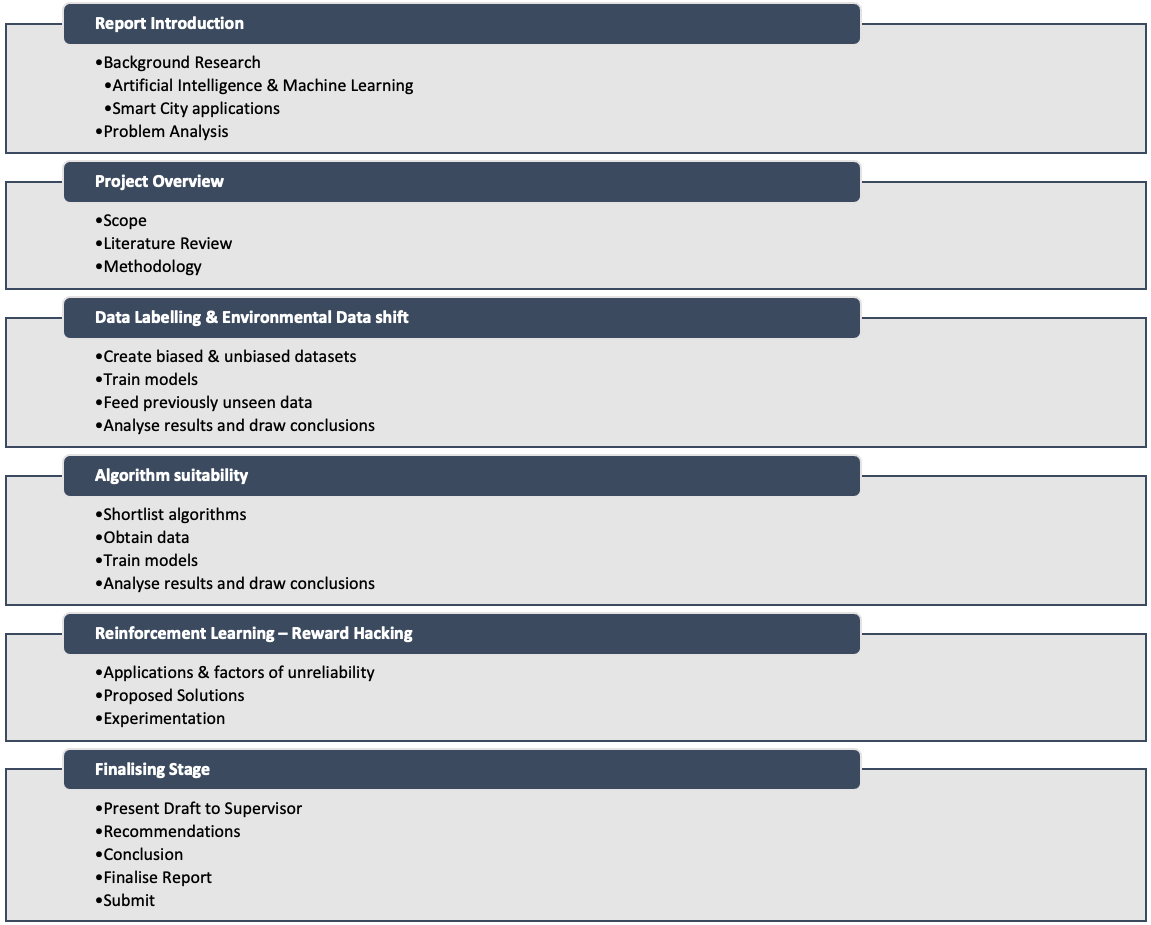
\includegraphics[width=1.2\textwidth]{milestones.png}
    \caption{Major and Minor Milestones}
    \label{fig:milestones}
\end{figure}

\subsection{Stage One: Report Introduction}
To prevent project delays, the report will be started early to shift focus on technical aspects during the closing stages of this project. 
Therefore, the introductory components will be completed prior to the start of semester as depicted in the schedule.
This introductory stage of the project involves research and analysis into the unreliability in Artificial Intelligence and Machine Learning. 
Potential causes are investigated with respect to Smart City applications before a problem is clearly defined.

\subsection{Stage Two: Project Overview}
After conducting background research on the causes of unreliability, a project scope is developed. Here literature review is performed
on the potential solutions in order to develop a suitable methodology to form the basis of this project.

\subsection{Stage Three: Data Labelling \& Environmental Data shift}
As mentioned in the methodology, the first technical stage involves investigating how biased data labelling will affect the ML model in unseen environments.  
First, a dataset is obtained from online sources and altered to create bias. The models are then trained using both the biased and original datasets. 
Environmental Datashift is simulated by feeding the model data which is of a similar nature but different to the training data. 
This means the labels will remain the same but the data istelf will be different. Finally, after testing each model's ability to generalize, we can analyse the results and draw conclusions.
Recommendations will also be made. 

\subsection{Stage Four: Algorithm Suitability}
In this stage, multiple algorithms are used to train a single dataset to determine algorithm suitability for specific applications.
After models have been trained, accuracy as well as other evaluation metrics are obtained and analysed to  draw conclusions. Recommendations will then be made.

\subsection{Stage Five: Reinforcement Learning – Reward Hacking}
The final technical stage of this project involves performing research into the applications and causes of reward hacking in reinforcement learning models. 
Literature Review is performed to determine current solutions and experimentation will be performed to evaulate various performances. 

\subsection{Stage Six: Finalising Stage}
Finally, after all stages have been completed, a draft report is produced and sent to my supervisor for review. 
Final recommendations and conclusions are drawn up before supervisor feedback and other issues will be addressed.
A second draft is then sent to my supervisor for review. After finalising, the final report will be submitted on 31 May 2021 as per schedule.

\section{Resources}
\subsection{Academic Supervisor – Diep Nguyen}
My academic supervisor, Diep Nguyen, is highly knowledgeable in the field of Machine Learning. 
Therefore, regular consultation would be a good idea to gather advice and guidance on topic related matters as well as suggestions on research content and experimentation. 

\subsection{Literature}
Literature such as journals and articles will be sourced from reliable sources such as IEEE, AMC, and Google Scholar. 
Various video tutorials may also be taken advantage of from platforms such as YouTube. 

\subsection{Technical Tools}
Experiments performed in this project will be completed using the Python programming language. 
This is due to the availability of many useful packages and its popularity within the data science community results in an abundance of available documentation and tutorials. 
Some of the packages we have access to are NumPy for mathematical operations such as arrays and matrices, Matplotlib for plotting and data visualisation, pandas for data analysis and manipulation, and scikit-learn for machine learning \cite{Justsajid}. 
There are many available deep learning libraries available such as Keras, TensorFlow and PyTorch. 
While they all have their pros and cons, PyTorch is preferred for this project due to its low-level nature allowing for experimentation \cite{deepsense}. 

\section{Uncertainties \& Risk Control}
See \hyperref[sec:app3]{Appendix 3} for a detailed Risk Assessment.

\subsection{Non-Technical}
Some non-technical risks and uncertainties could affect the completion of this project. 
The biggest risks in this project are those that would prevent successful completion. 
There lies the risk of failing to complete the project due to delays and difficulties in completing milestones. 
To prevent this, buffer periods have been added to the schedule. These periods will allow me to catch up to schedule if I do find myself falling behind. 
If the buffer periods aren’t required, I will find myself ahead of schedule which is another benefit.

The next greatest threat to this project is an inadequate understanding of the critical components involved in this project. 
It is essential to adhere to the schedule, revisit reliable sources and consult my supervisor as soon as possible in these circumstances. 

Another risk is the loss of work and other saved data due to uncontrollable reasons such as computer failures. 
To prevent this, all work will be saved to OneDrive (cloud storage). 

There is also the uncertainty of ideas and general direction of the research report. 
In these cases, example or past reports can be viewed. Many high-quality reports (Distinction and High Distinction) reports can be found on the UTS Library website and are available for download. 
My supervisor should also be consulted for advice. 

Finally, due to the global COVID-19 pandemic, there is the potential risk of infection to myself, supervisor or other university peers. 
The best course of prevention is to eliminate the possibility of transmitting the virus. Therefore, all work on this project will be carried out at home. 
Potential face-to-face meetings will be replaced with virtual meetings through platforms such as zoom. 
In the rare case where I do find myself at university or if it is absolutely necessary to enter campus, I will ensure to wear a mask and sanitize regularly.

\subsection{Technical}
There will always be risks and uncertainties involved in any stage of an ML or DL project. 
Specifically, in the case of reliability, it is possible that the problem is misdiagnosed, and the cause/s are not clearly or correctly identified. 
In such cases, we would be attempting to develop a solution or optimise current algorithms against problems that simply don’t exist. 
Therefore, it is essential to look deeply into problems to gain a good understanding of problems. 

During the experimentation stage, there are risks that the dataset is already biased which would be caused by an overrepresentation of one party/feature over the other. 
It is essential to understand the deployment environment, consider all variables and balance accordingly. \cite{sires} 

Other risks when it comes to data are false data being used in training, or errors in the labelling of data. 
This would indicate that training data is not representative of real-world data. 

There is also the risk of improper training of the model which could lead to over or underfitting of the training dataset. 
This could be the result of insufficient knowledge and understanding of training algorithms. 
It is critical to carefully read into all resources to limit misunderstanding. 

The most important uncertainty of this project is the effectiveness of proposed solutions and algorithms using real-world data. 
It would be inefficient to collect real-world data and perform experiments within the given timeframe of this project. 
Consequently, all results and conclusions will be drawn from the dataset used in simulations. 
There is the fair chance a dataset shift could be observed if our models are to be used against real-world data \cite{gupta}.

There are also social threats in the form of evasion attacks or adversarial inputs that can have an effect on ML models. 
Adversarial inputs involve an external party or attacker who has the ability to manipulate data may do so with malicious intent. 
This would result in the model making incorrect predications often with high confidence \cite{gupta}. 
A remedy to this is adversarial training where adversarial examples are created and used during training of the model. 
Although effective, it is impossible to protect against all evasion attacks as hackers continue to grow in creativity in terms of hacking ability. 
However, this is an insignificant risk and only has a slim chance of affecting this project.

\newpage
\section{Communication Plan}
The following communication plan has been developed between myself and my academic supervisor Diep Nguyen. 
I am planning to maintain contact with Diep on a fortnightly basis on various project-related matters.
I have also planned online meetings to discuss revisions for major milestones. No other stakeholders are involved in this project.

\begin{table}[h]
    \centering
    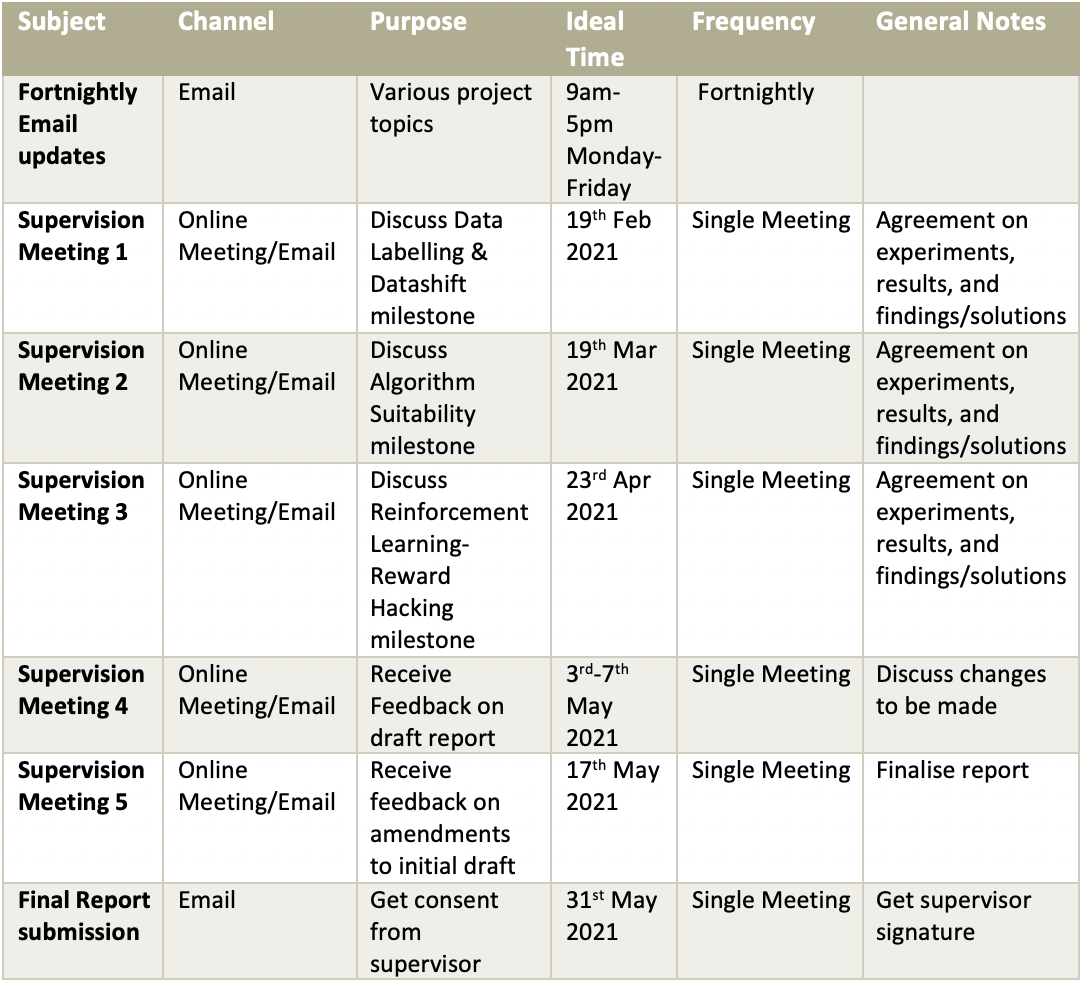
\includegraphics[width=\textwidth]{communication plan.png}
    \caption{Communiation Plan}
    \label{tab:comm}
\end{table}

%% Progress Statement
\chapter{Progress Statement}
\enlargethispage{\baselineskip}
Coming into this project I had little to no real and/or valuable experience or understanding of Artificial Intelligence or Machine Learning. 
I have spent a respectable amount of time throughout this semester researching and learning not only the basic concepts but also begun looking into factors of unreliability and thinking of a suitable methodology for the capstone project.
As the objective started to become clearer, and with the guidance of my supervisor, I have made changes to initial thought processes and potential ideas for this project. 
I believe the methodology I have prepared and the goals I have set are realistic and achievable in terms of time frame and ability. 
While it is easy to get carried away with the excitement and intriguingness of AI/ML, it is important to propose goals that are feasible.

I spent quite some time researching about various platforms to perform these experiments on. Some options were, TensorFlow, PyTorch, Keras, and MATLAB. 
Since I had very little experience with ML as a whole, I had no skill advantage with either of these, meaning I would need to learn the basic concepts either way. 
While I have experience in both Python and MATLAB, based on community opinions on forums I have chosen to go with PyTorch as the availability of information and support online is far greater than MATLAB.

This project will run in accordance with the schedule prepared in \hyperref[sec:app2]{Appendix 2}. The first activities in the proposed schedule do not start until January of 2021. 
Having done a significant amount of research during this semester already, the first stages of the report have fundamentally been completed and will only require small modifications. 
This leaves more time for the experimentation stages of this project.

\newpage
My productivity has been limited over this semester as a consequence of a larger than expected study load. 
While I undertook four subjects this semester, next semester I will only undertake two subjects including this capstone. 
As a result, the majority of my time will be spent on this project, therefore I anticipate an increase in productivity and may even find myself ahead of schedule. 
This would give me additional time to consult my supervisor to increase the quality of my project. 

\renewcommand{\bibname}{References}
\bibliographystyle{ieeetr}
\bibliography{references}

\newgeometry{top=10mm, bottom=30mm}  
\chapter{Appendix}
\section{Appendix 1: Communication Log}
\begin{table}[H]
    \centering
    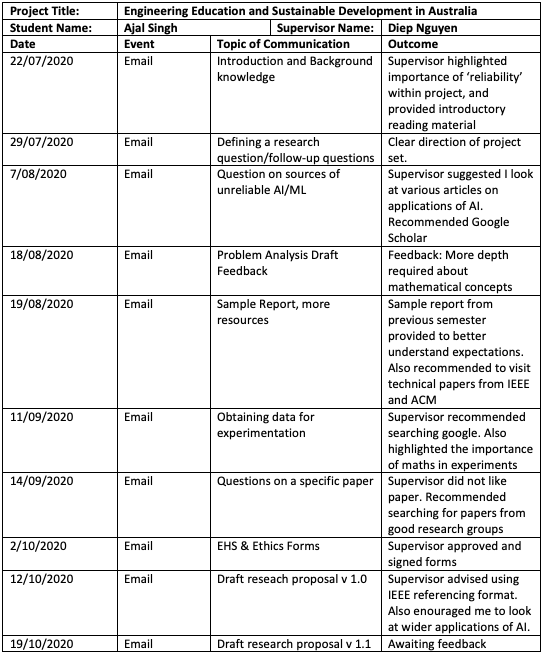
\includegraphics[width=0.9\textwidth]{communication log.png}
    \caption{Communication Log}
    \label{fig:comm log}
\end{table}
\restoregeometry

\begin{landscape}
    \section{Appendix 2: Gantt Chart \& Milestones}
    \label{sec:app2}
    \begin{figure}[H]
        \centering
        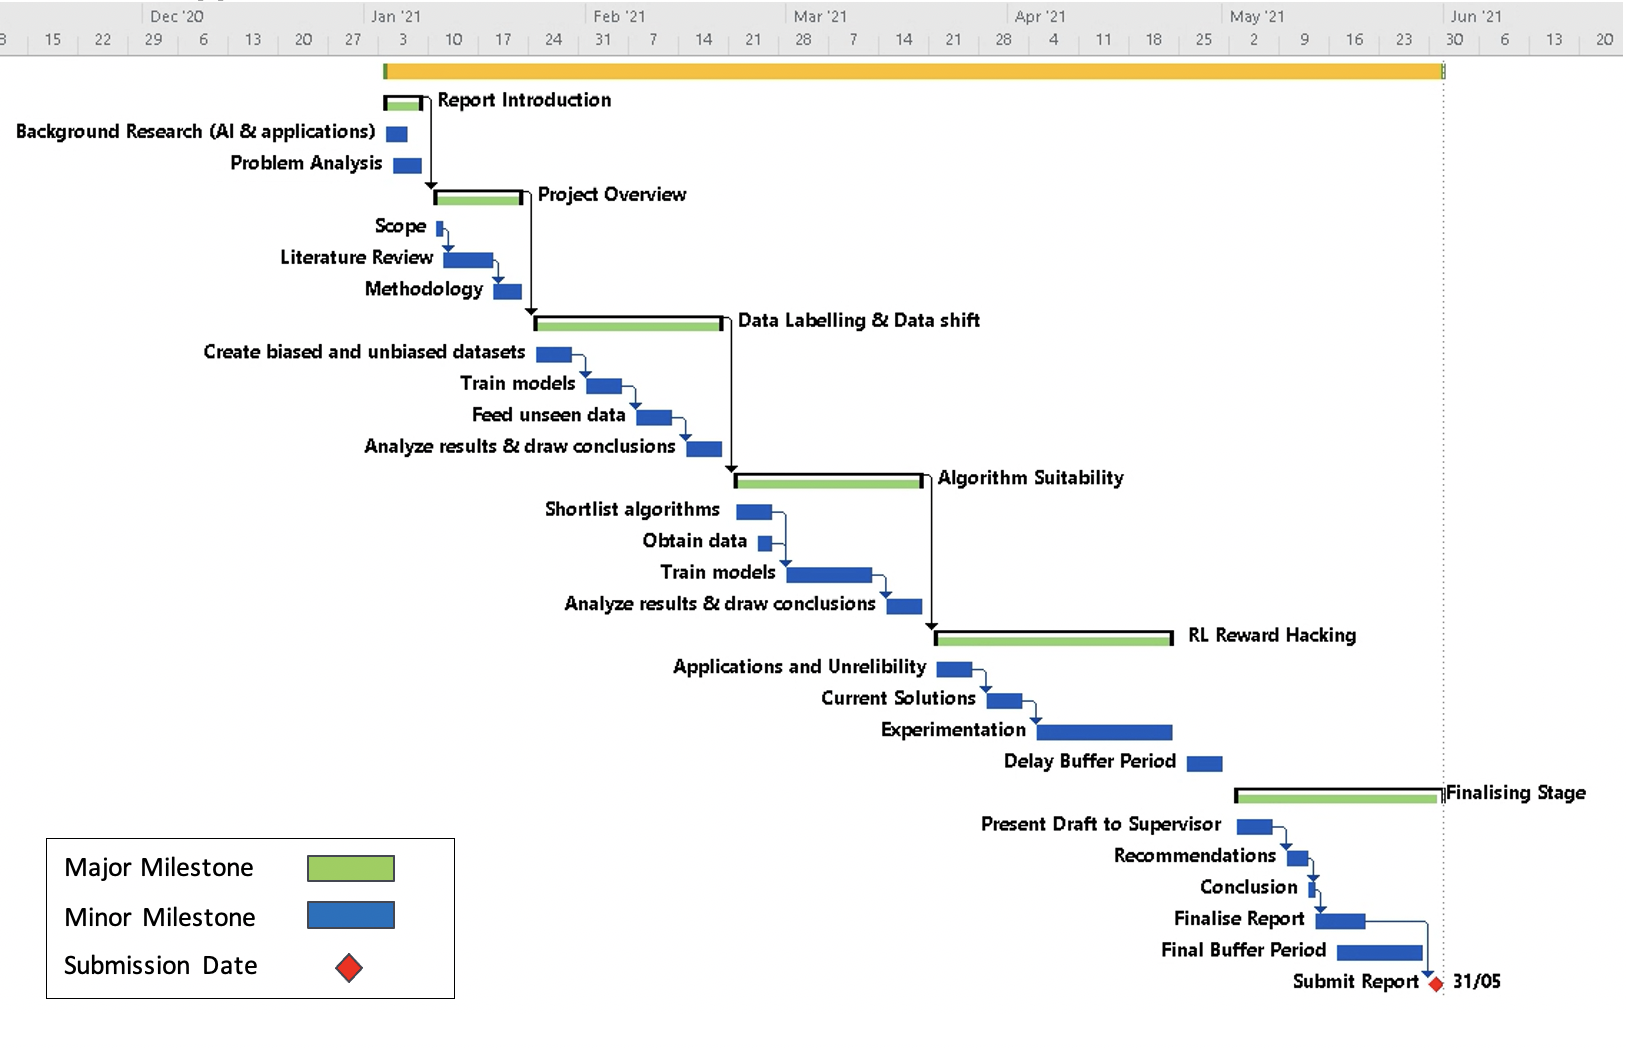
\includegraphics[width=1.2\textwidth]{gantt chart.png}
        \caption{Gantt Chart}
        \label{fig:gantt}
    \end{figure}
\end{landscape}

\newgeometry{top=30mm, bottom=30mm} 
\begin{table}[H]
    \centering
    \hspace*{-1.5cm}  
    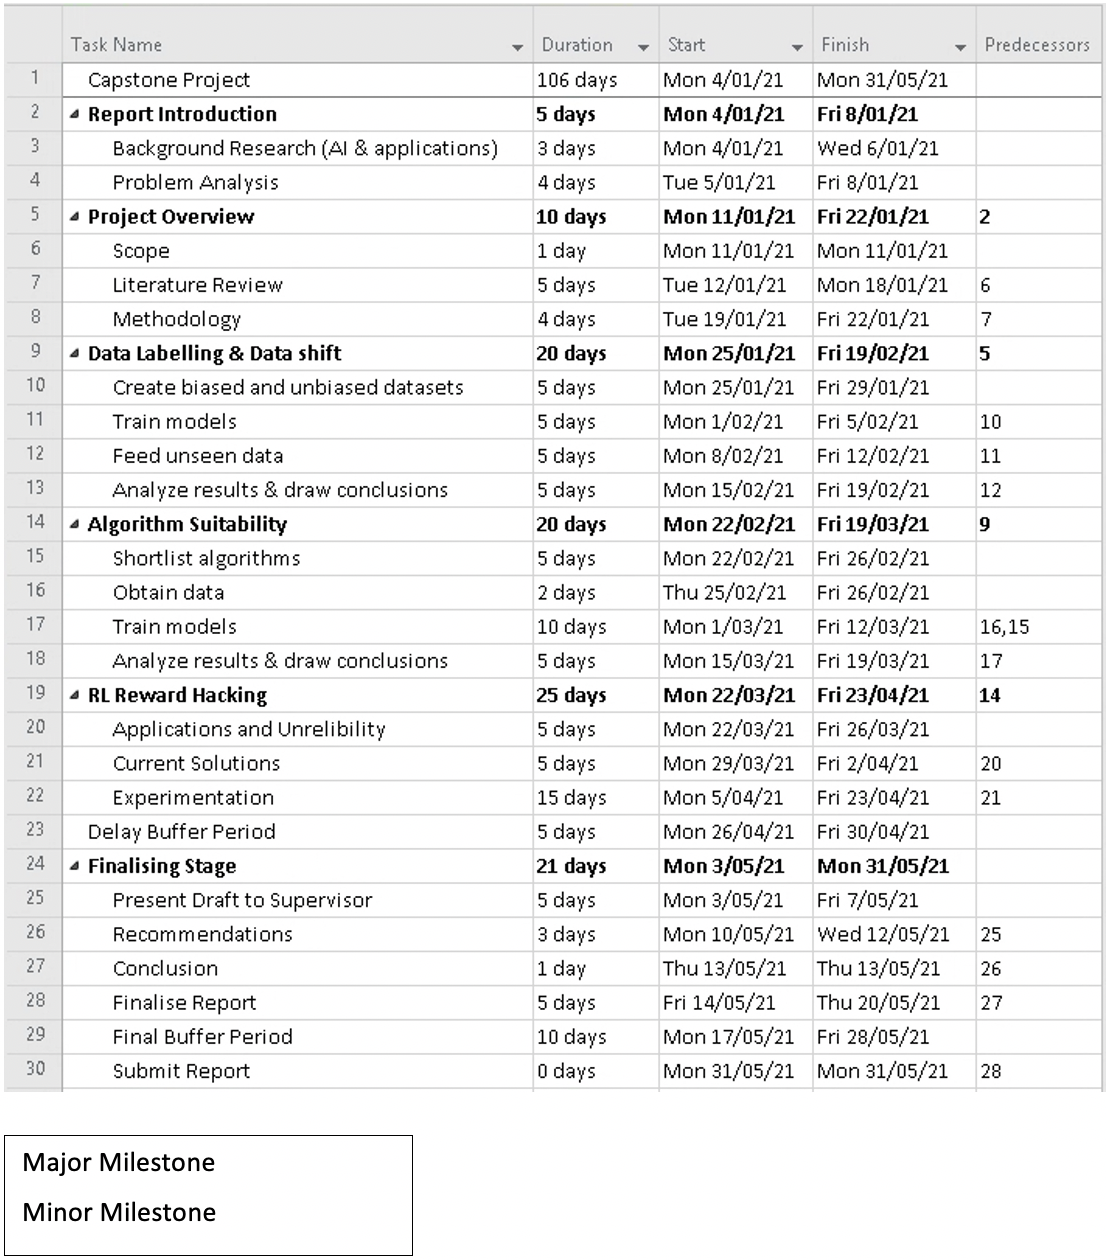
\includegraphics[width=1.2\textwidth]{schedule.png}
    \caption{Project Schedule}
    \label{fig:schedule}
\end{table}
\restoregeometry

\section{Appendix 3: Risk Assessment}
\label{sec:app3}
\begin{table}[H]
    \centering
    \hspace*{-1.5cm}  
    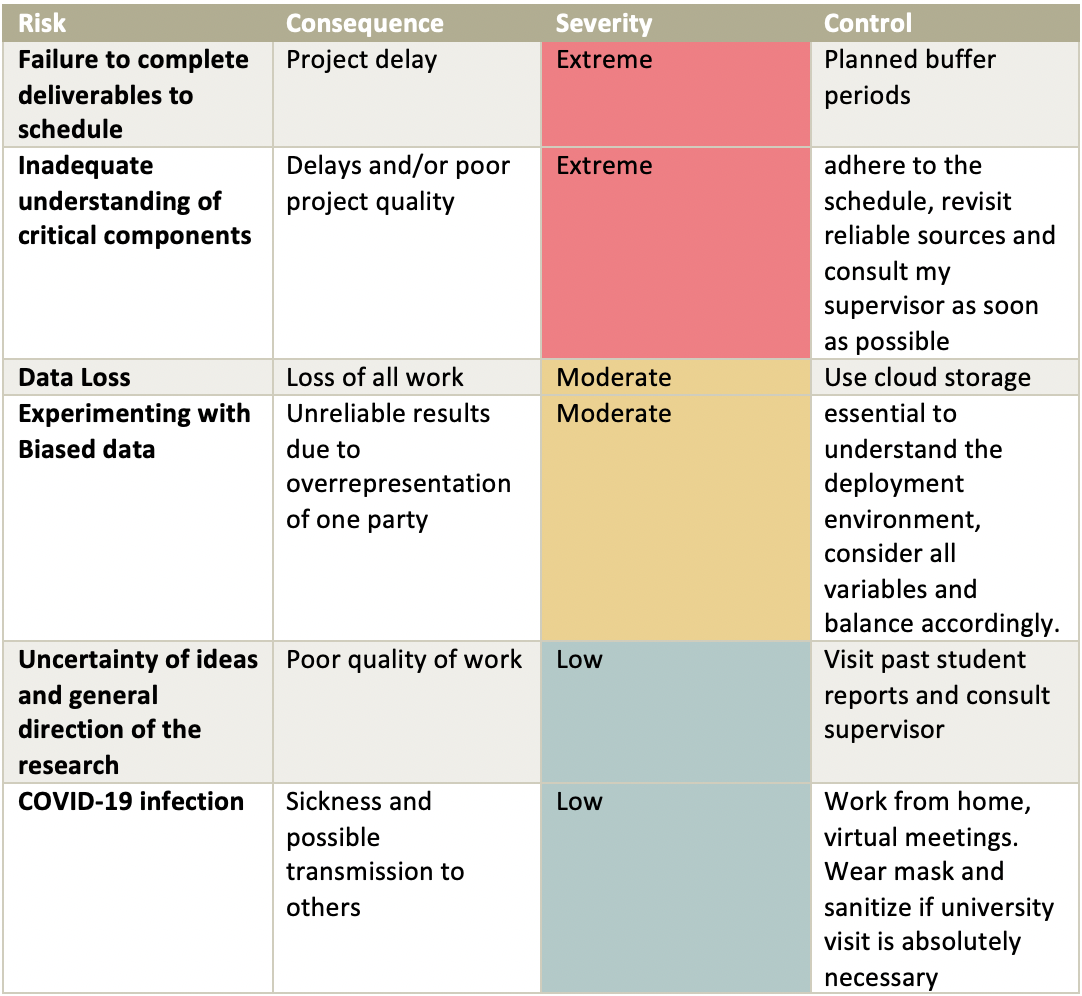
\includegraphics[width=1.2\textwidth]{risk assessment.png}
    \caption{Risk Assessment}
    \label{tab:Risk}
\end{table}

\end{document}